\documentclass[11pt]{exam}

\usepackage{amsmath}
\usepackage{graphicx}
\usepackage{geometry}
\usepackage{etoolbox}
\BeforeBeginEnvironment{choices}{\par\nopagebreak\minipage{\linewidth}}
\AfterEndEnvironment{choices}{\endminipage}
\geometry{
a4paper,
total={185mm,257mm},
left=10mm,
top=25mm,
bottom=10mm
}

\begin{document}
\setlength{\voffset}{-0.5in}
\setlength{\headsep}{5pt}

\fbox{\fbox{\parbox{8cm}{\centering
\vspace{2mm}
Testat - Versuch J - Ultraschall 
\vspace{2mm}
}}}
\hspace{2mm}
\makebox[0.25\textwidth]{Name:\enspace\hrulefill} \hspace{5mm}
\makebox[0.2\textwidth]{Datum:\enspace\hrulefill}
\vspace{4mm}

\begin{questions}

\question In der Graphik (beliebige Einheiten) wird die Periodendauer wiedergegeben durch ... ? 

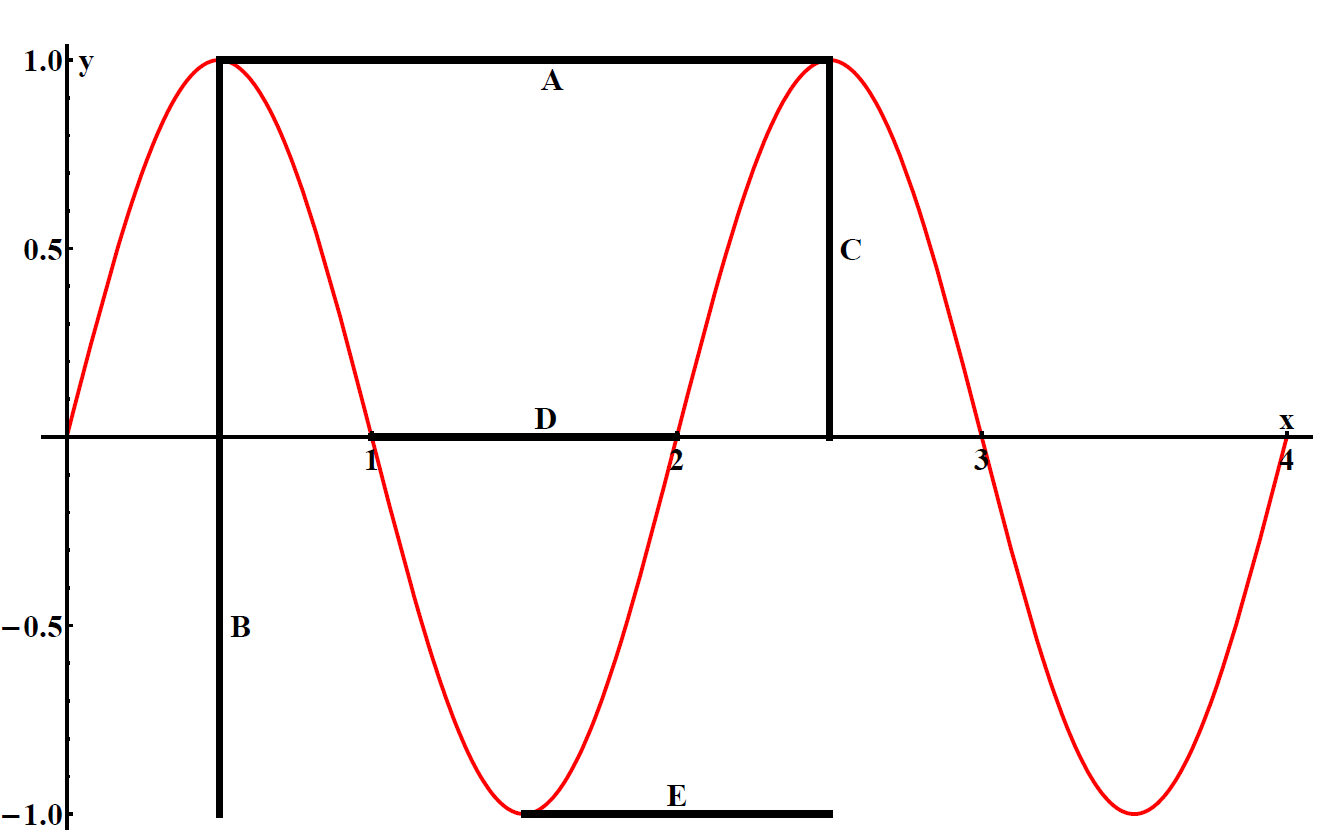
\includegraphics[width=0.4\textwidth]{images/Sinuskurve.png}

\begin{choices}
	\choice Linie C
	\choice Linie B
	\choice Linie E
	\choice Linie A (correct)
	\choice Linie D
\end{choices}

\vspace{3mm}\question Welche der folgenden Formeln für die Schallgeschwindigkeit ist richtig?( \( c \) Schallgeschwindigkeit, \(T \) Periodendauer, \( f \) Frequenz, \( \lambda \) Wellenlänge)

\begin{choices}
	\choice \( c=\frac{T}{\lambda} \)
	\choice \( c=T \cdot f \)
	\choice \( c=f \cdot \lambda \) (correct)
	\choice \( c=\frac{f}{\lambda} \)
	\choice \( c=T \cdot \lambda \)
\end{choices}

\vspace{3mm}\question Eine Schallwelle in Luft mit der Periodendauer \( T= \mathrm{1~s} \) hat eine Wellenlänge \( \lambda \) von ...?

\begin{choices}
	\choice 3,43 m
	\choice 343 km/h
	\choice 34,3 m
	\choice 343 m (correct)
	\choice 34,3 km/h
\end{choices}

\vspace{3mm}\question Die Schallgeschwindigkeit...

\begin{choices}
	\choice ist im Vakuum größer als in Luft, da die Luftmoleküle die Schallübertragung dämpfen
	\choice Keine Antwort ist richtig.
	\choice ist vom Übertragenden Medium unabhängig
	\choice hängt von der Amplitude der Schallwelle ab
	\choice ist bei zwei Schallwellen mit unterschiedlicher Frequenz gleich, wenn sie sich im gleichen Medium ausbreiten. (correct)
\end{choices}

\vspace{3mm}\question Welche Aussage zu Schallwellen ist richtig?

\begin{choices}
	\choice Die Wellenlänge bezeichnet die Zeit zwischen zwei Schalldruckmaxima an einem festen Ort.
	\choice Die Schalldruckamplitude einer Schallwelle bezeichnet die Differenz zwischen maximalem und minimalem Schalldruck.
	\choice Bei Longitudinalwellen erfolgt die Auslenkung der Teilchen parallel zur Ausbreitungsrichtung. (correct)
	\choice Die Wellenlänge wird in der Einheit Hertz (Hz) angegeben.
	\choice Die Frequenz bezeichnet die Strecke zwischen zwei Schalldruckmaxima.
\end{choices}

\vspace{3mm}\end{questions}

\end{document}
